\documentclass[a4paper]{article}
\usepackage[left=2.1cm, right=2.1cm, top=2.1cm]{geometry}
\usepackage{lipsum}
\usepackage{tikzpagenodes}
\usepackage{pgfplots}
\usepackage{tikz}
\usepackage{tikz-3dplot}
\usetikzlibrary{arrows,decorations.pathmorphing,backgrounds,positioning,fit,matrix}
\pgfplotsset{compat=1.8}
\usepackage{graphics} % for pdf, bitmapped graphics files
\usepackage{epsfig} % for postscript graphics files
\usepackage[colorlinks=true,citecolor=green]{hyperref}
\usepackage{cite}
\usepackage{amsmath,amssymb,amsfonts}
\usepackage{algorithmic}
\usepackage{graphicx}
\usepackage{url}
\usepackage{cite}
\usepackage{bm}
\usepackage{pbox}
\usepackage{siunitx,booktabs,etoolbox}
\usepackage{ulem}
\usepackage[framed,numbered,autolinebreaks,useliterate]{mcode}
\usepackage{filecontents}
%\usepackage{bigfoot} % to allow verbatim in footnote


\def\BibTeX{{\rm B\kern-.05em{\sc i\kern-.025em b}\kern-.08em
    T\kern-.1667em\lower.7ex\hbox{E}\kern-.125emX}}
\begin{filecontents*}{box.m}
clear
close all
Q=Box3D;
plot3(Q(1,:),Q(2,:),Q(3,:),'.'),
axis equal
axis([-1 1 -1 1 -1 5])
xlabel('x')
ylabel('y')
zlabel('z')
\end{filecontents*}
\begin{filecontents*}{cube.m}
x = 0:0.1:5;
y = 0:0.1:5;
pt = [x repmat(x(end), 1, numel(y)) fliplr(x) repmat(x(1), 1, numel(y)); repmat(y(1), 1, numel(y)) y repmat(y(end), 1, numel(y)) fliplr(y)];
pt = [pt;ones(1,size(pt,2))];  
\end{filecontents*}

\begin{filecontents*}{ipm1.m}
clc;close all;clear all;
I = imread('Tiles_perspective_distort.png');
I = im2double(I);
h = figure;
imshow(I);
[x,y] = ginput(4);
q = round([x y]');
q = [q;ones(1,4)];
I = drawlines(I,q,[[1 2];[3 4];[1 4];[2 3]]);
imshow(I);
\end{filecontents*}

%\begin{filecontents*}{box.mat}
%clear
%close all
%Q=Box3D;
%%plot3(Q(1,:),Q(2,:),Q(3,:),’.’),
%%axis equal
%%axis([-1 1 -1 1 -1 5])
%%xlabel(’x’)
%%ylabel(’y’)
%%zlabel(’z’)
%\end{filecontents*}

\begin{document}

\title{Exercise on Homogenous Coordinates \& Projective Geometry}
%\author{xiahaa@space.dtu.dk}
\maketitle%%

In this exercise, we will work with a few assignments related to projective camera model and homogeneous coordinates.

\section{Homogeneous Coordinates}
\paragraph{Q1:} Transforming the following homogeneous coordinates to their corresponding inhomogeneous coordinates
\begin{align}
\begin{matrix}
\left[ \begin{matrix} 3 \\ 4 \\ 1\end{matrix}\right], & 
\left[ \begin{matrix} 4 \\ 6.5 \\ 0.5 \end{matrix}\right], &
\left[ \begin{matrix} 5 \\ 2 \\ 0.1 \end{matrix}\right], &
\left[ \begin{matrix} 10 \\ 100 \\ 20 \end{matrix}\right], &
\left[ \begin{matrix} 0.1 \\ 0.2 \\ 100 \end{matrix}\right]
\end{matrix} \nonumber
\end{align} 

\paragraph{Q2:} Transforming the following homogeneous coordinates to their corresponding inhomogeneous coordinates
\begin{align}
\begin{matrix}
\left[ \begin{matrix} 3 \\ 4 \\ 1 \\ 0.1 \end{matrix}\right], & 
\left[ \begin{matrix} 4 \\ 6.5 \\ 0.5 \\ 2 \end{matrix}\right], &
\left[ \begin{matrix} 5 \\ 2 \\ 0.1 \\ 3 \end{matrix}\right], &
\left[ \begin{matrix} 10 \\ 100 \\ 20 \\ 1  \end{matrix}\right], &
\left[ \begin{matrix} 0.1 \\ 0.2 \\ 100 \\ 10 \end{matrix}\right]
\end{matrix} \nonumber
\end{align} 

\paragraph{Q3:} 
Find the line which passes the following two 2D points: $$\mathbf{p}_1=(1,2)^{T},\ \mathbf{p}_2=(5,3.5)^{T}$$

\paragraph{Q4:} Compute the distance of point $\mathbf{p}_1=(7.5,3.6)^{T}$ to the line you find in \textbf{Q3}.

\paragraph{Q5:} Find the intersection of two lines given as
$$
\mathbf{l}_1 = [1,\ 1,\ -1]^{T},\ \mathbf{l}_2 = [-1,\ 3,\ -4]^{T},
$$

\section{2D Transformation}
To give your an better illustration of 2D transformation, we will work with a simple square. The square can be generated using the following code:
\lstinputlisting[caption = {Sample code from Matlab}]{cube.m}

\paragraph{Q6:} Given a matrix $\mathbf{A}$ given as
$$
\mathbf{A} = \left[\begin{matrix}
0.8660  &  0.5000     &    2.0000 \\ 
-0.5000  &  0.8660  &       -2.0000 \\
0 &  0 &     1.0000 \end{matrix}\right]
$$
By applying the transformation of $\mathbf{A}$ to the square, what will you get, plot them in one figure and explain what is the effect by multiplying the matrix A? Are there any invariants conserved?

\paragraph{Q7:} Try with $\mathbf{A}$ as 
$$
\mathbf{A} = \left[\begin{matrix}
0.1732  &  0.1000     &    2.0000 \\ 
-0.1000  &  0.1732  &       -2.0000 \\
0 &  0 &     1.0000 \end{matrix}\right]
$$
Plot and explain what is the effect by multiplying the matrix A? Are there any invariants conserved?

\paragraph{Q8:} Try with another $\mathbf{A}$ as
$$
\mathbf{A} = \left[\begin{matrix}
0.5000  &  0.3000     &    2.0000 \\ 
0.1000  &  1.2000  &       -2.0000 \\
0 &  0 &     1.0000 \end{matrix}\right]
$$
Plot and observe which invariant is still preserved?

%\section{Pinhole Camera Model}
%Here you should exercise in computing with the pinhole camera model. For you to have something to 'photograph'. a sample object is supplied in the accompanying file \textit{Box3D}. To see this box try the following script:
%\lstinputlisting{box.m}
%\paragraph{Q9:} Start with the projection matrix as 
%$$
%\mathbf{K} = \left[\begin{matrix}
%f  &  0     &    0 \\ 
%0  &  f  &       0 \\
%0 &  0 &     1 \end{matrix}\right]=
%\left[\begin{matrix}
%1  &  0     &    0 \\ 
%0  &  1  &       0 \\
%0 &  0 &     1 \end{matrix}\right]
%$$
%Please apply the projection and then plot the image you get. 
%Are those orthogonal lines are still orthogonal? Why? When you finish this, try to add some radial distortion given as
%$$
%[a_1,\ a_2,\ a_3,\ a_4] = [0.2, 0.1, 0, 0]
%$$
%Plot again and observe what has changed.

\section{Inverse Perspective Mapping}
\paragraph{Q9:} Here you will work on how to remove the perspective effect by using the vanishing line and 2D transformation. Use the following code to load and display the image you will work:
\lstinputlisting{ipm1.m}
Then click on the displayed image to obtain the coordinates of four points you clicked. \textbf{q} will contain their homogeneous coordinates. You should work from here.

In this attachment, you will find two supplementary files.
\begin{itemize}
\item \textbf{drawlines.m} - draw lines on image I.
\item \textbf{warpping.m} - warp image I by transformation matrix $\mathbf{H}$. So after you find $\mathbf{H}$, call this function to get the resultant image.
\end{itemize}
%If you succeed, you will have a similar image like
\begin{figure*}[!b]
\centering
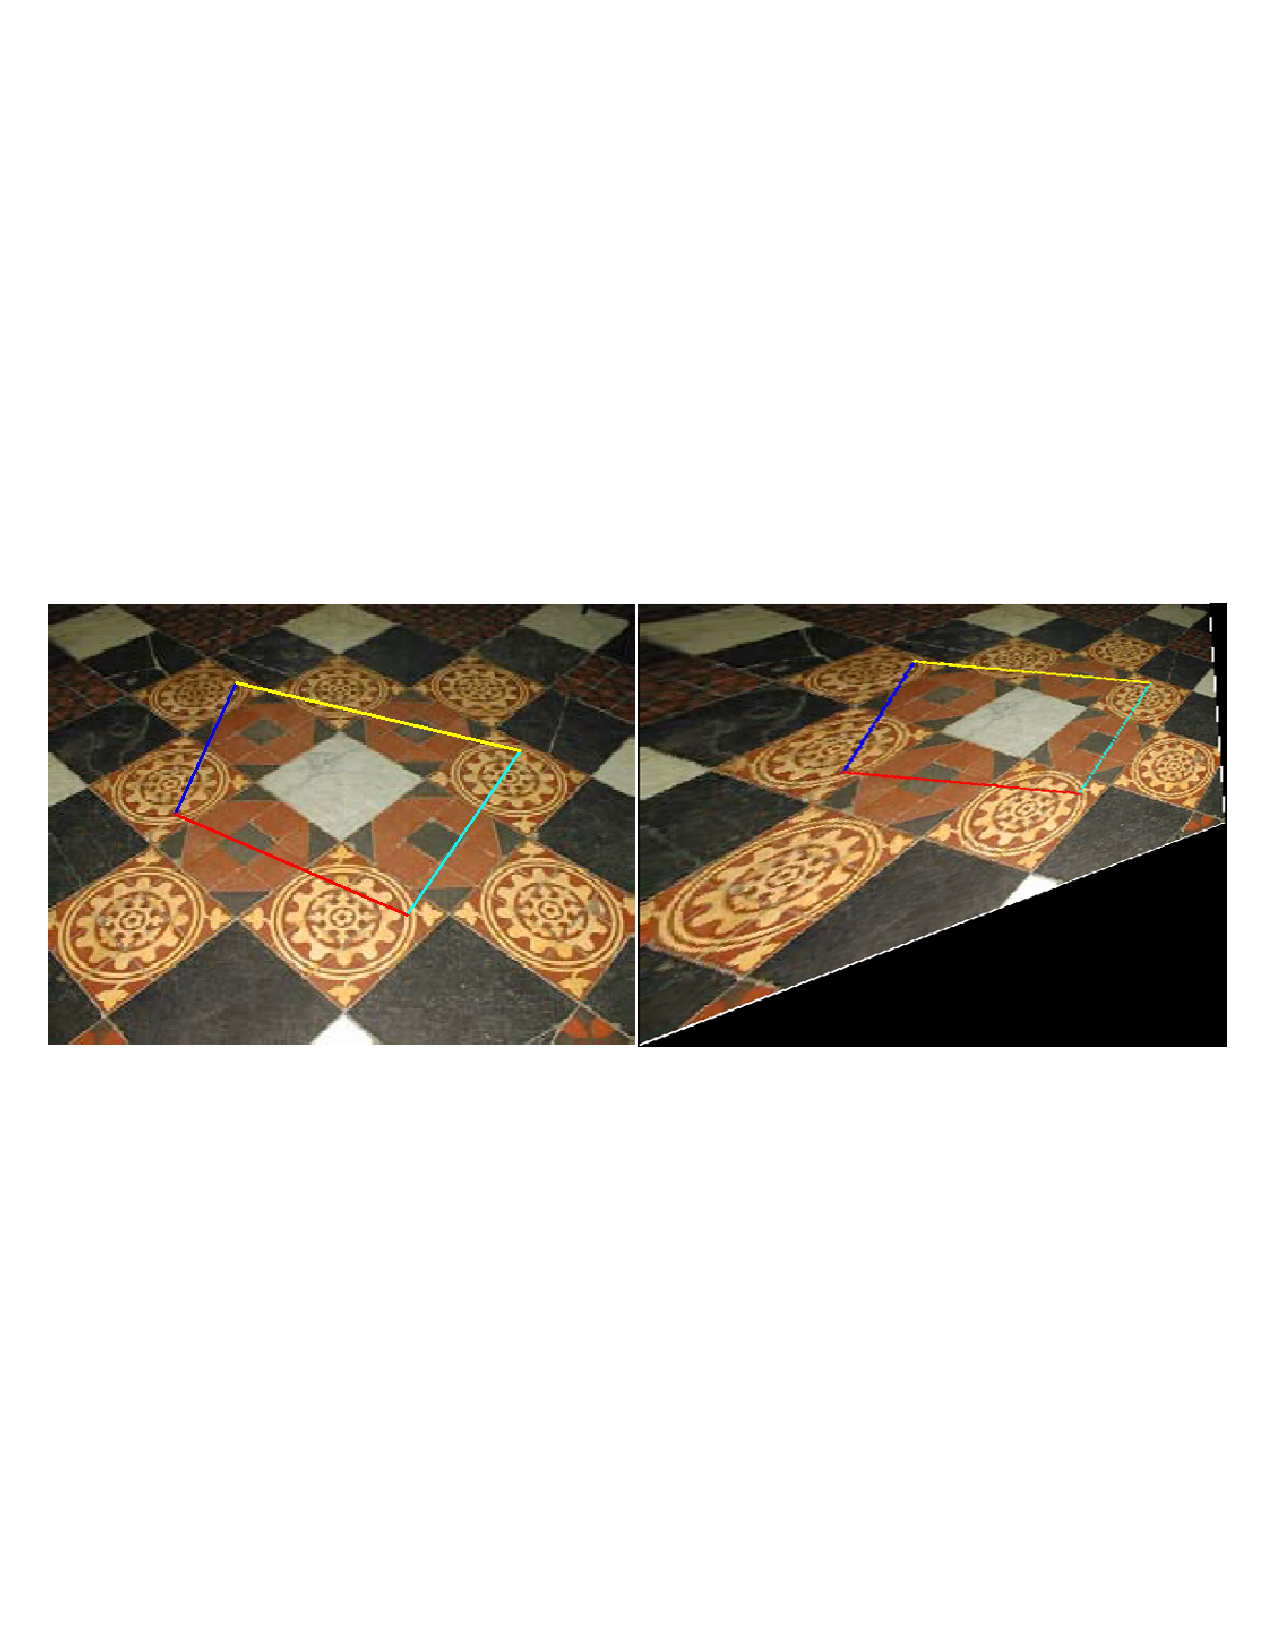
\includegraphics[scale=0.6]{figures/ipm}
\caption{Illustration of the inverse perspective mapping.}
\end{figure*}


 
\bibliography{hand_eye_calibration} 
\bibliographystyle{ieeetr}

\end{document}